\documentclass[10pt]{article}
\usepackage[a4paper,landscape,hmargin=0.9cm,vmargin=0.7cm]{geometry}
\usepackage[T1]{fontenc}
\usepackage{helvet}
\renewcommand{\familydefault}{\sfdefault}
\usepackage{xcolor}
\usepackage{tikz}
\usepackage{adjustbox}
\usetikzlibrary{arrows.meta,calc,shapes.geometric}
\pagestyle{empty}
\setlength{\parindent}{0pt}

\definecolor{stF}{HTML}{E9F0F8}  \definecolor{stL}{HTML}{3D6FA8}   % data stores
\definecolor{aiC}{HTML}{B4500F}                                     % AI component tag
\definecolor{txG}{HTML}{555555}                                     % secondary text
\definecolor{lnG}{HTML}{8A8A8A}                                     % lane borders

\newcommand{\sm}[1]{{\scriptsize\color{txG}#1}}
\newcommand{\tag}[1]{\,{\setlength{\fboxsep}{1pt}\fcolorbox{aiC}{white}{\textcolor{aiC}{\tiny\bfseries #1}}}}
\newcommand{\ML}{\tag{ML}}
\newcommand{\LLM}{\tag{LLM}}

\tikzset{
  comp/.style ={draw=black!75, fill=white, align=center, font=\footnotesize,
                inner sep=2.5pt, line width=0.5pt},
  store/.style={cylinder, shape border rotate=90, aspect=0.16, draw=stL, fill=stF,
                align=center, font=\footnotesize, inner sep=2pt, line width=0.6pt},
  lane/.style ={draw=lnG, line width=0.6pt},
  lanet/.style={font=\footnotesize\bfseries, anchor=north west, inner sep=0pt},
  lanen/.style={font=\scriptsize, text=txG, anchor=north east, inner sep=0pt},
  flow/.style ={-{Stealth[length=2mm]}, line width=0.65pt},
  ro/.style   ={-{Stealth[length=2mm]}, line width=0.65pt, dash pattern=on 2.5pt off 1.5pt},
  assoc/.style={line width=0.45pt, dotted},
  al/.style   ={font=\scriptsize, text=txG, fill=white, inner sep=1pt},
  pics/actor/.style={code={
      \draw[line width=0.6pt] (0,0.2) circle (0.075);
      \draw[line width=0.6pt] (0,0.125) -- (0,-0.07);
      \draw[line width=0.6pt] (-0.12,0.06) -- (0.12,0.06);
      \draw[line width=0.6pt] (0,-0.07) -- (-0.09,-0.24) (0,-0.07) -- (0.09,-0.24);
  }}
}
\newcommand{\comp}[5]{\node[comp, text width=#4cm-5pt, minimum height=#5cm] (#1) at (#2,#3)}

\begin{document}
{\Large\bfseries Collections 360 \textbar{} System Architecture (shipped)}\hfill{\normalsize\bfseries Team: Straw Hats \,|\, Build phase, 4 Oct 2026}\\[2pt]
{\small Kondameedi Srujan Raj, D Varshith Reddy, G Swachatha, T Sreenidhi}\hfill{\small CIBC Collections Hackathon, IIIT Hyderabad \,|\, Use case: Next Best Action}\\[-6pt]
{\scriptsize\color{txG}Layer ownership: L1--L2 by Kondameedi Srujan Raj \,|\, L3--L4 by D Varshith Reddy}\\[-4pt]
\rule{\textwidth}{0.6pt}\\[2pt]

\begin{adjustbox}{max width=\textwidth, max totalheight=\dimexpr\textheight-1.6cm\relax, center}
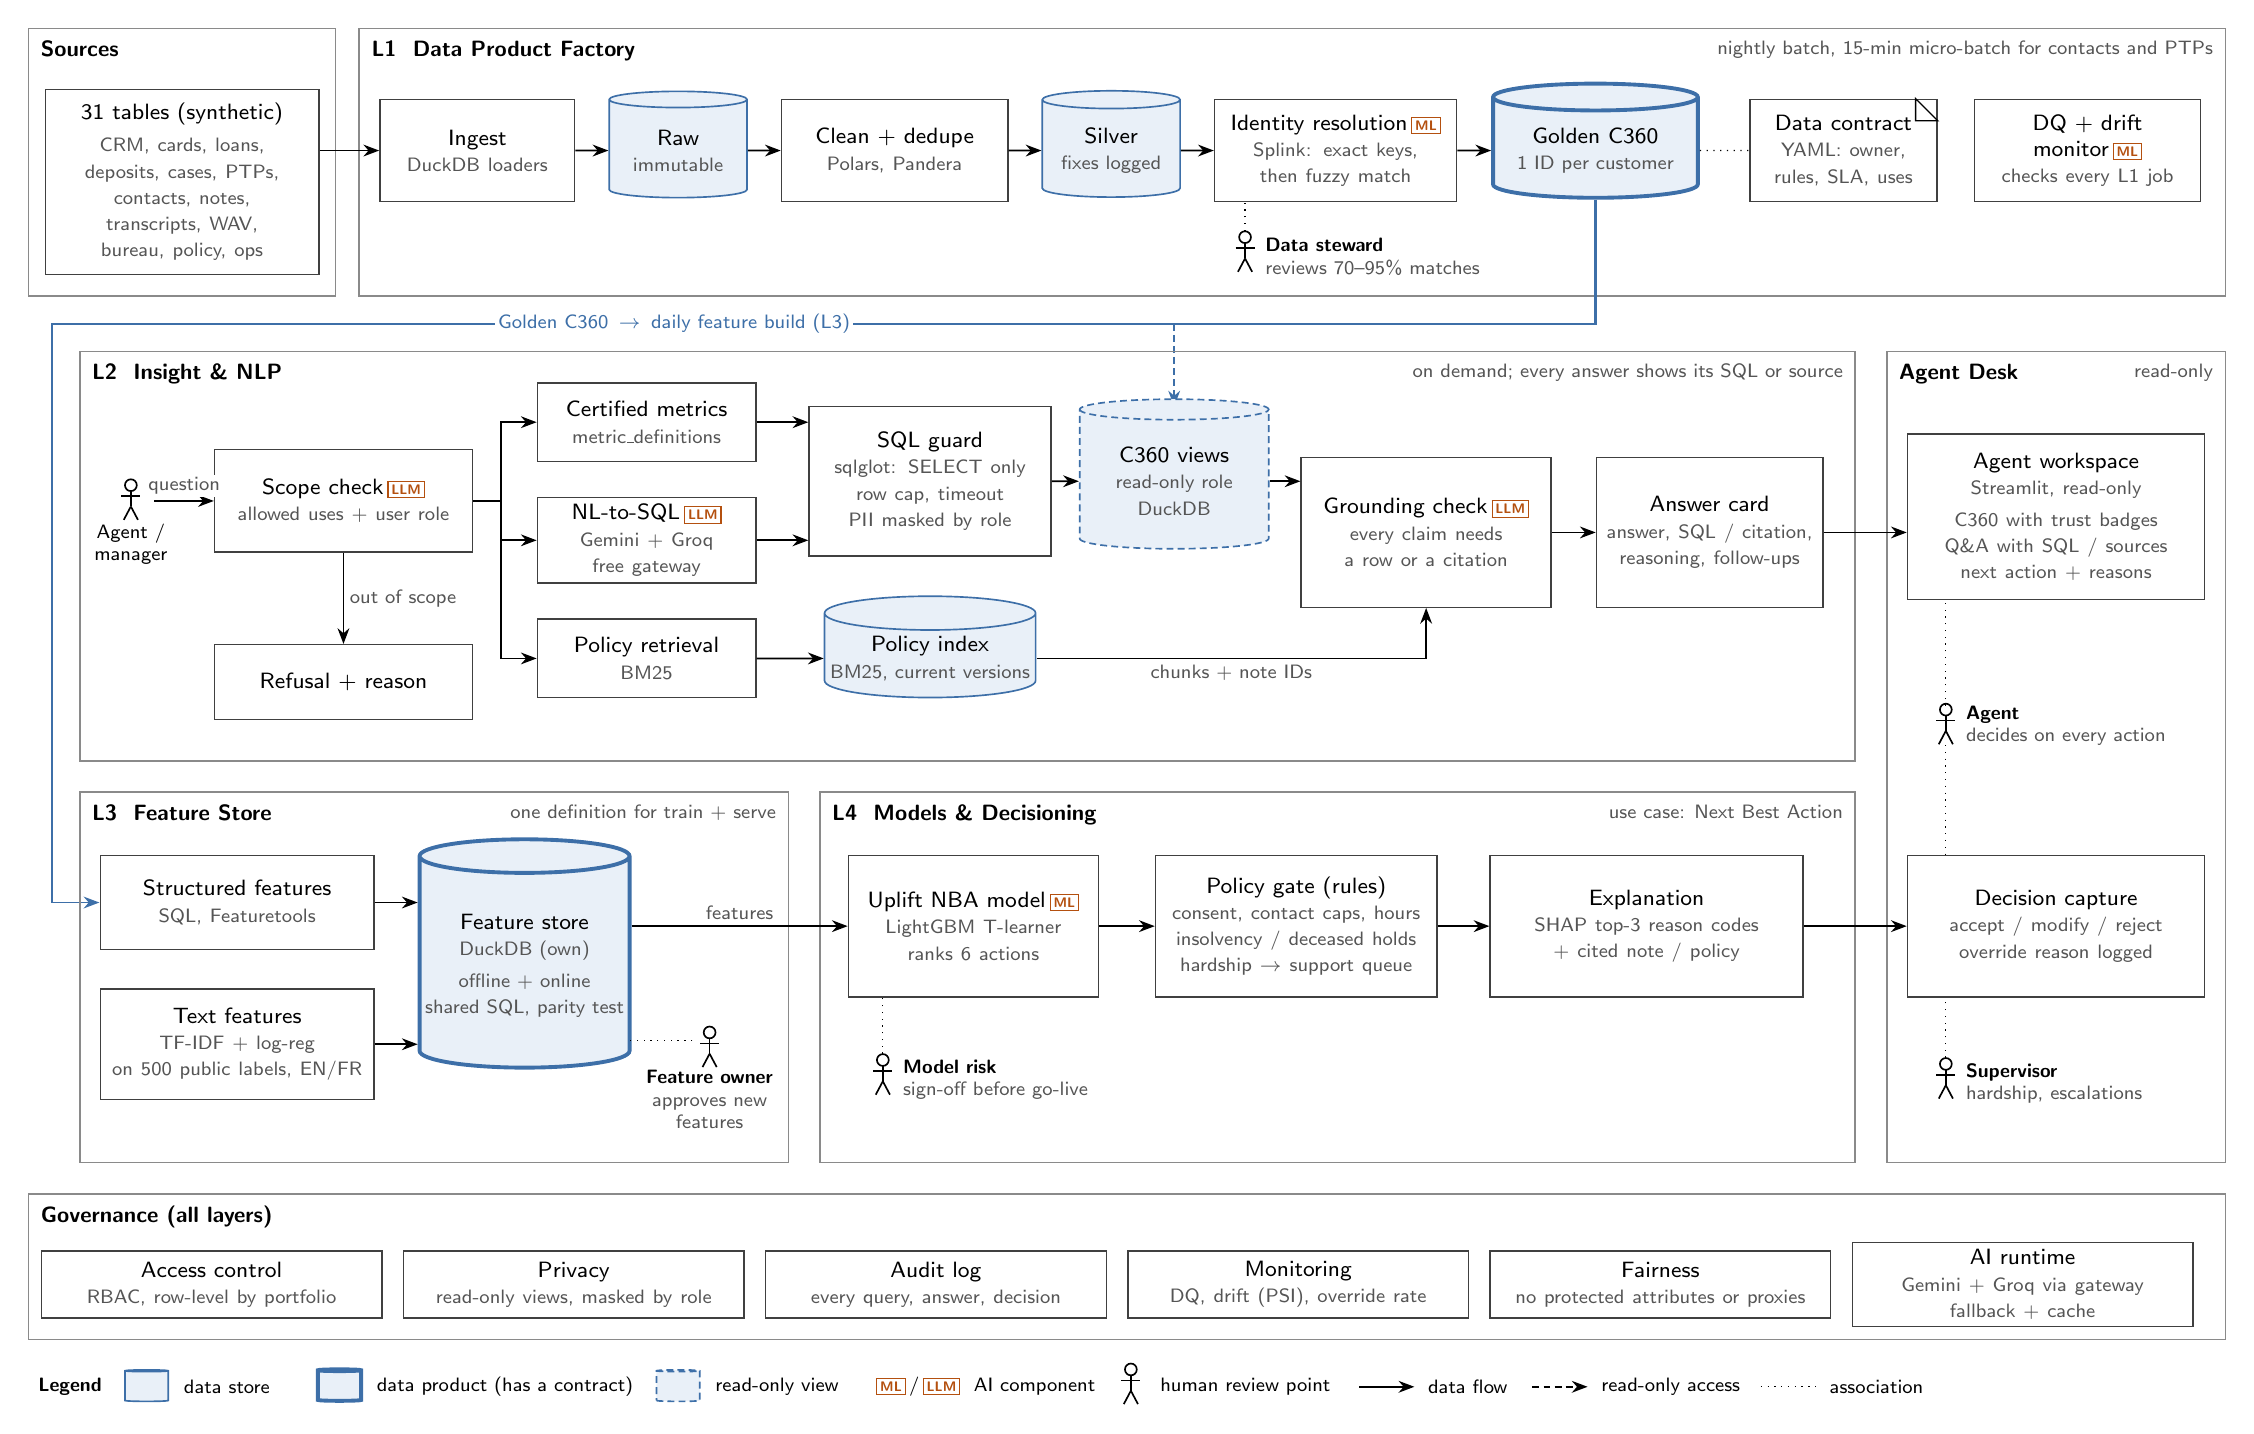
\begin{tikzpicture}[x=1cm,y=1cm]

% =================== SOURCES ===================
\draw[lane] (0,0) rectangle (3.9,-3.4);
\node[lanet] at (0.15,-0.15) {Sources};
\node[comp, text width=3.3cm, minimum height=2.35cm] (src) at (1.95,-1.95)
 {31 tables (synthetic)\\[2pt]\sm{CRM, cards, loans,}\\\sm{deposits, cases, PTPs,}\\\sm{contacts, notes,}\\\sm{transcripts, WAV,}\\\sm{bureau, policy, ops}};

% =================== L1 ===================
\draw[lane] (4.2,0) rectangle (27.9,-3.4);
\node[lanet] at (4.35,-0.15) {L1 \ Data Product Factory};
\node[lanen] at (27.75,-0.15) {nightly batch, 15-min micro-batch for contacts and PTPs};

\node[comp, text width=2.3cm, minimum height=1.3cm] (in)  at (5.7,-1.55)  {Ingest\\\sm{DuckDB loaders}};
\node[store, minimum width=1.75cm, minimum height=1.35cm] (raw) at (8.25,-1.55) {Raw\\\sm{immutable}};
\node[comp, text width=2.7cm, minimum height=1.3cm] (std) at (11.0,-1.55) {Clean + dedupe\\\sm{Polars, Pandera}};
\node[store, minimum width=1.75cm, minimum height=1.35cm] (sil) at (13.75,-1.55) {Silver\\\sm{fixes logged}};
\node[comp, text width=2.9cm, minimum height=1.3cm] (idr) at (16.6,-1.55) {Identity resolution\ML\\\sm{Splink: exact keys,}\\\sm{then fuzzy match}};
\node[store, minimum width=2.6cm, minimum height=1.45cm, line width=1.4pt] (gold) at (19.9,-1.55) {Golden C360\\\sm{1 ID per customer}};
\node[comp, text width=2.2cm, minimum height=1.3cm] (con) at (23.05,-1.55) {Data contract\\\sm{YAML: owner,}\\\sm{rules, SLA, uses}};
\draw[line width=0.5pt, fill=white] ($(con.north east)+(-0.28,0)$) -- ($(con.north east)+(0,-0.28)$) -- ($(con.north east)+(-0.28,-0.28)$) -- cycle;
\node[comp, text width=2.7cm, minimum height=1.3cm] (mon) at (26.15,-1.55) {DQ + drift monitor\ML\\\sm{checks every L1 job}};
\draw[flow] (src.east |- in.west) -- (in.west);
\draw[flow] (in) -- (raw); \draw[flow] (raw) -- (std); \draw[flow] (std) -- (sil); \draw[flow] (sil) -- (idr); \draw[flow] (idr) -- (gold);
\draw[assoc] (gold) -- (con);

\pic at (15.45,-2.85) {actor};
\draw[assoc] (15.45,-2.57) -- (15.45,-2.2);
\node[anchor=west, font=\scriptsize, align=left, inner sep=0pt] at (15.7,-2.9) {\textbf{Data steward}\\\color{txG}reviews 70--95\% matches};

% ---- C360 distribution line ----
\draw[line width=0.8pt, stL] (gold.south) -- (19.9,-3.75) -- (0.3,-3.75) -- (0.3,-11.1);
\node[al, text=stL] at (8.2,-3.75) {Golden C360 \,$\rightarrow$\, daily feature build (L3)};
\draw[flow, stL] (0.3,-11.1) -- (0.9,-11.1);
\draw[ro, stL] (14.55,-3.75) -- (14.55,-4.8);

% =================== L2 ===================
\draw[lane] (0.65,-4.1) rectangle (23.2,-9.3);
\node[lanet] at (0.8,-4.25) {L2 \ Insight \& NLP};
\node[lanen] at (23.05,-4.25) {on demand; every answer shows its SQL or source};

\pic at (1.3,-6.0) {actor};
\node[font=\scriptsize, align=center, inner sep=0pt] at (1.3,-6.55) {Agent /\\manager};
\node[comp, text width=3.1cm, minimum height=1.3cm] (sc) at (4.0,-6.0) {Scope check\LLM\\\sm{allowed uses + user role}};
\node[comp, text width=3.1cm, minimum height=0.95cm] (rf) at (4.0,-8.3) {Refusal + reason};
\draw[flow] (1.6,-6.0) -- node[al, above=1pt]{question} (sc.west);
\draw[flow] (sc.south) -- node[al, right=1pt]{out of scope} (rf.north);

\node[comp, text width=2.6cm, minimum height=1.0cm] (mt) at (7.85,-5.0) {Certified metrics\\\sm{metric\_definitions}};
\node[comp, text width=2.6cm, minimum height=1.0cm] (ns) at (7.85,-6.5) {NL-to-SQL\LLM\\\sm{Gemini + Groq}\\\sm{free gateway}};
\node[comp, text width=2.6cm, minimum height=1.0cm] (rt) at (7.85,-8.0) {Policy retrieval\\\sm{BM25}};
\draw[line width=0.65pt] (sc.east) -- (6.0,-6.0);
\foreach \n in {mt,ns,rt} { \draw[flow] (6.0,-6.0) |- (\n.west); }

\node[comp, text width=2.9cm, minimum height=1.9cm] (gd) at (11.45,-5.75) {SQL guard\\\sm{sqlglot: SELECT only}\\\sm{row cap, timeout}\\\sm{PII masked by role}};
\node[store, minimum width=2.5cm, minimum height=1.25cm] (ix) at (11.45,-8.0) {Policy index\\\sm{BM25, current versions}};
\draw[flow] (mt.east) -- (gd.west |- mt.east);
\draw[flow] (ns.east) -- (gd.west |- ns.east);
\draw[flow] (rt) -- (ix);

\node[store, minimum width=2.4cm, minimum height=1.9cm, dash pattern=on 2.5pt off 1.5pt] (vw) at (14.55,-5.75) {C360 views\\\sm{read-only role}\\\sm{DuckDB}};
\draw[flow] (gd) -- (vw);

\node[comp, text width=3.0cm, minimum height=1.9cm] (gr) at (17.75,-6.4) {Grounding check\LLM\\\sm{every claim needs}\\\sm{a row or a citation}};
\draw[flow] (vw.east) -- (gr.west |- vw.east);
\draw[flow] (ix.east) -| node[al, pos=0.25, below=1pt]{chunks + note IDs} (gr.south);

\node[comp, text width=2.7cm, minimum height=1.9cm] (an) at (21.35,-6.4) {Answer card\\\sm{answer, SQL / citation,}\\\sm{reasoning, follow-ups}};
\draw[flow] (gr) -- (an);

% =================== L3 ===================
\draw[lane] (0.65,-9.7) rectangle (9.65,-14.4);
\node[lanet] at (0.8,-9.85) {L3 \ Feature Store};
\node[lanen] at (9.5,-9.85) {one definition for train + serve};

\node[comp, text width=3.3cm, minimum height=1.2cm] (sf) at (2.65,-11.1) {Structured features\\\sm{SQL, Featuretools}};
\node[comp, text width=3.3cm, minimum height=1.4cm] (tv) at (2.65,-12.9) {Text features\\\sm{TF-IDF + log-reg}\\\sm{on 500 public labels, EN/FR}};
\node[store, minimum width=2.6cm, minimum height=2.9cm, line width=1.4pt] (fs) at (6.3,-11.9) {Feature store\\\sm{DuckDB (own)}\\[2pt]\sm{offline + online}\\\sm{shared SQL, parity test}};
\draw[flow] (sf.east) -- (fs.west |- sf.east);
\draw[flow] (tv.east) -- (fs.west |- tv.east);
\pic at (8.65,-12.95) {actor};
\draw[assoc] (8.43,-12.85) -- (7.6,-12.85);
\node[font=\scriptsize, align=center, inner sep=0pt] at (8.65,-13.6) {\textbf{Feature owner}\\\color{txG}approves new\\\color{txG}features};

% =================== L4 ===================
\draw[lane] (10.05,-9.7) rectangle (23.2,-14.4);
\node[lanet] at (10.2,-9.85) {L4 \ Models \& Decisioning};
\node[lanen] at (23.05,-9.85) {use case: Next Best Action};

\node[comp, text width=3.0cm, minimum height=1.8cm] (md) at (12.0,-11.4) {Uplift NBA model\ML\\\sm{LightGBM T-learner}\\\sm{ranks 6 actions}};
\node[comp, text width=3.4cm, minimum height=1.8cm] (pg) at (16.1,-11.4) {Policy gate (rules)\\\sm{consent, contact caps, hours}\\\sm{insolvency / deceased holds}\\\sm{hardship $\rightarrow$ support queue}};
\node[comp, text width=3.8cm, minimum height=1.8cm] (ex) at (20.55,-11.4) {Explanation\\\sm{SHAP top-3 reason codes}\\\sm{+ cited note / policy}};
\draw[flow] (fs.east |- md.west) -- node[al, above=1pt]{features} (md.west);
\draw[flow] (md) -- (pg); \draw[flow] (pg) -- (ex);
\pic at (10.85,-13.3) {actor};
\draw[assoc] (10.85,-13.02) -- (10.85,-12.3);
\node[anchor=west, font=\scriptsize, align=left, inner sep=0pt] at (11.1,-13.35) {\textbf{Model risk}\\\color{txG}sign-off before go-live};

% =================== AGENT DESK ===================
\draw[lane] (23.6,-4.1) rectangle (27.9,-14.4);
\node[lanet] at (23.75,-4.25) {Agent Desk};
\node[lanen] at (27.75,-4.25) {read-only};

\node[comp, text width=3.6cm, minimum height=2.1cm] (ws) at (25.75,-6.2) {Agent workspace\\\sm{Streamlit, read-only}\\[2pt]\sm{C360 with trust badges}\\\sm{Q\&A with SQL / sources}\\\sm{next action + reasons}};
\node[comp, text width=3.6cm, minimum height=1.8cm] (dc) at (25.75,-11.4) {Decision capture\\\sm{accept / modify / reject}\\\sm{override reason logged}};
\draw[flow] (an.east) -- (ws.west |- an.east);
\draw[flow] (ex.east) -- (dc.west);
\pic at (24.35,-8.85) {actor};
\draw[assoc] (24.35,-8.6) -- (24.35,-7.25);
\draw[assoc] (24.35,-9.1) -- (24.35,-10.5);
\node[anchor=west, font=\scriptsize, align=left, inner sep=0pt] at (24.6,-8.85) {\textbf{Agent}\\\color{txG}decides on every action};
\pic at (24.35,-13.35) {actor};
\draw[assoc] (24.35,-13.07) -- (24.35,-12.3);
\node[anchor=west, font=\scriptsize, align=left, inner sep=0pt] at (24.6,-13.4) {\textbf{Supervisor}\\\color{txG}hardship, escalations};

% =================== GOVERNANCE ===================
\draw[lane] (0,-14.8) rectangle (27.9,-16.65);
\node[lanet] at (0.15,-14.95) {Governance (all layers)};
\foreach \i/\t in {
 0/{Access control\\\sm{RBAC, row-level by portfolio}},
 1/{Privacy\\\sm{read-only views, masked by role}},
 2/{Audit log\\\sm{every query, answer, decision}},
 3/{Monitoring\\\sm{DQ, drift (PSI), override rate}},
 4/{Fairness\\\sm{no protected attributes or proxies}},
 5/{AI runtime\\\sm{Gemini + Groq via gateway}\\\sm{fallback + cache}}}
 { \node[comp, text width=4.15cm, minimum height=0.85cm] at (2.325+\i*4.6,-15.95) {\t}; }

% =================== LEGEND ===================
\begin{scope}[shift={(0,-17.25)}]
\node[font=\scriptsize\bfseries, anchor=west] at (0,0) {Legend};
\node[store, minimum width=0.55cm, minimum height=0.4cm] at (1.5,0) {};
\node[font=\scriptsize, anchor=west] at (1.85,0) {data store};
\node[store, minimum width=0.55cm, minimum height=0.4cm, line width=1.4pt] at (3.95,0) {};
\node[font=\scriptsize, anchor=west] at (4.3,0) {data product (has a contract)};
\node[store, minimum width=0.55cm, minimum height=0.4cm, dash pattern=on 2.5pt off 1.5pt] at (8.25,0) {};
\node[font=\scriptsize, anchor=west] at (8.6,0) {read-only view};
\node[font=\scriptsize, anchor=west] at (10.6,0) {\ML\,/\LLM\ \ AI component};
\pic at (14.0,0.02) {actor};
\node[font=\scriptsize, anchor=west] at (14.25,0) {human review point};
\draw[flow] (16.9,0) -- (17.6,0); \node[font=\scriptsize, anchor=west] at (17.65,0) {data flow};
\draw[ro] (19.1,0) -- (19.8,0); \node[font=\scriptsize, anchor=west] at (19.85,0) {read-only access};
\draw[assoc] (22.0,0) -- (22.7,0); \node[font=\scriptsize, anchor=west] at (22.75,0) {association};
\end{scope}
\end{tikzpicture}
\end{adjustbox}
\end{document}
